
\documentclass[a4paper,12pt]{article}
\usepackage{graphicx}
\usepackage{amssymb}					%Calls AMS symbols
\usepackage{amsthm}	

\begin{document}

\section{Introduction}

To simulate population dynamics we use ODE predator-prey models (see \ref{sec:s3_model_derivation}), expressed in the form: 

\begin{eqnarray}
\frac{d\chi_{0}}{dt} &=& A\chi_0(1-\chi_0) - B\chi_1F(\chi_0,\chi_1) \label{eq:general_simple_form1} \\
\frac{d\chi_{1}}{dt} &=& -\chi_1 + C\chi_1F(\chi_0,\chi_1) \label{eq:general_simple_form2}, 
\end{eqnarray}

where $\chi_1$ is the predator density, $\chi_0$ is the re-scaled prey density, $F(\chi_0,\chi_1)$ is the functional response (FR), and the parameters $A,B,C \in \mathbb{R}^+$. We use three different forms for the FR (see table \ref{table:response_interaction_table}) which gives three distinct simulation models.
\\
We use the metric for interaction strength defined by the elements of the \emph{interaction matrix} (IM):

\begin{equation}
\label{eq:IM_defined}
\alpha_{ij} = \frac{\partial}{\partial x_{j}}(\frac{\dot{x}_{i}}{x_{i}}),
\end{equation}  

where $i,j$ index the species, $x_i$ is the population density of species $i$, and $\dot{x}_i$ is its rate of change. Therefore the functional responses and interaction strengths are shown in table \ref{table:response_interaction_table}.

\begin{center}
\begin{table}[hb!]

    \begin{tabular}{| l | l | l | l |}

    \hline
    Response Type & $F(X_0,X_1)$ & $\alpha_{01}$ & $\alpha_{10}$ \\ \hline
    Linear & $X_0$ & $-B$ & $C$ \\ \hline
    Holling II & $\frac{X_0}{X_0 + D}$ & $\frac{-B}{X_0 + D} $ & $\frac{CD}{(X_0 + D)^2}$ \\ \hline
    Arditi-Michalski & $\frac{X_0/X_1}{X_1+DX_0}$ & $\frac{1}{(X_1+DX_0)^2}$ & $\frac{C(1-X_0)}{X_1(X_1+DX_0)}$ \\
    \hline
    \end{tabular}
    
\caption{Table showing the three types of functional response used, their expression in the reduced parameter space, and the corresponding interaction strengths (derived by applying expression \ref{eq:IM_defined} to equations \ref{eq:general_simple_form1},\ref{eq:general_simple_form2}).}
\label{table:response_interaction_table}    
\end{table}
\end{center}

\newpage

\begin{figure}[ht!]
\centering 
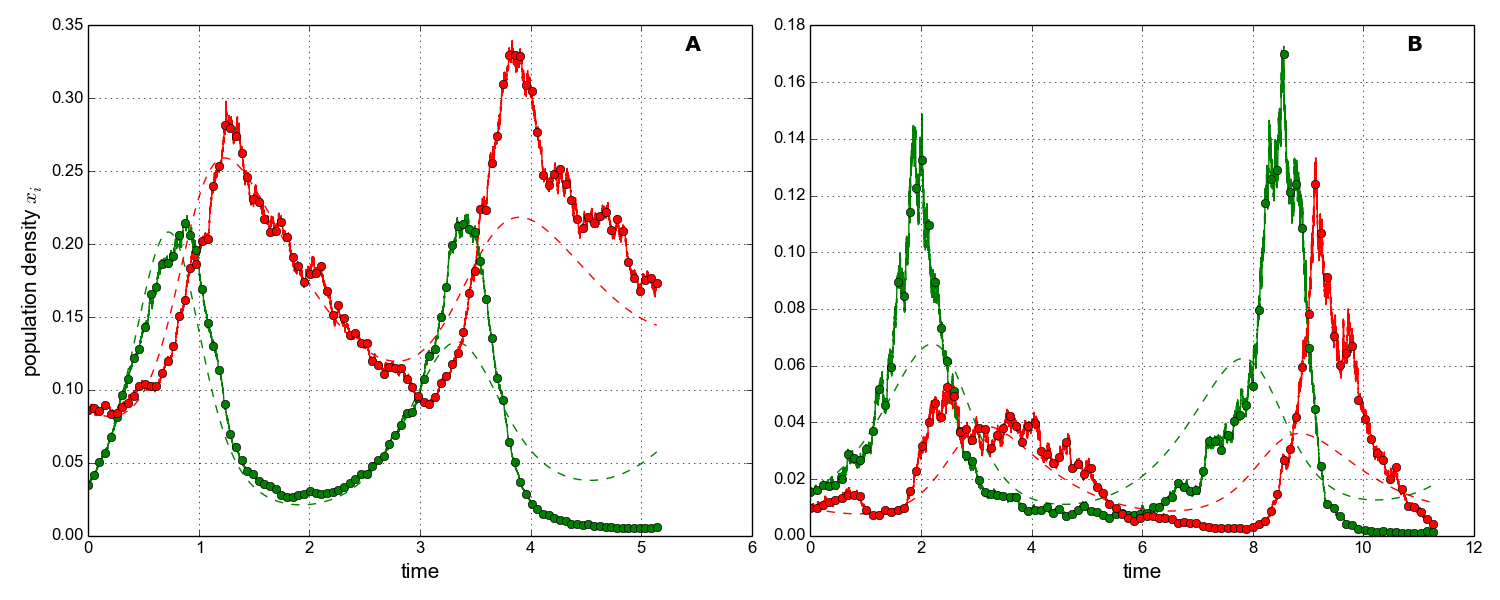
\includegraphics[width=\textwidth]{{{figures/example_dynamics_pID_0_and_87_noise_20.000000}}}
\caption{Examples dynamics with linear functional response. Panel A and B show dynamics for two different parameter sets. The dashed lines give the deterministic dynamics of predator and prey abundances. The solid lines show an instance of stochastic dynamics with $\sigma_{noise}=20$. The circles indicate 100 uniformly spaced samples taken from the dynamics, as is used for estmimation of inter-specific interaction strengths.}
\label{fig:example_linear_dynamics}
\end{figure}


\begin{figure}[hb!]
\centering 
\includegraphics[width=\textwidth]{{{figures/example_dynamics_HII_pID_0_and_1_noise_20.000000}}}
\caption{Examples dynamics with Holling type II functional response. The left hand panels show dynamics for two different parameter sets, as in figure \ref{fig:example_linear_dynamics}. The right hand panels shows the variation in the magnitude of the interaction strengths between the species during these simulations.} 
\label{fig:example_holling_dynamics}
\end{figure}

\newpage

\section{Functional Responses and interaction strengths}

For linear (Lotka-Volterra type) functional response gives constant interaction strengths. Whereas Holling II FR gives interaction strengths that are functions of prey density. It is also possible, using other FR forms to obtain interaction strengths that are mutlivariate functions of two or more species densities. In such cases interactions may not be strictly pairwise.

\begin{figure}[hb!]
\centering 
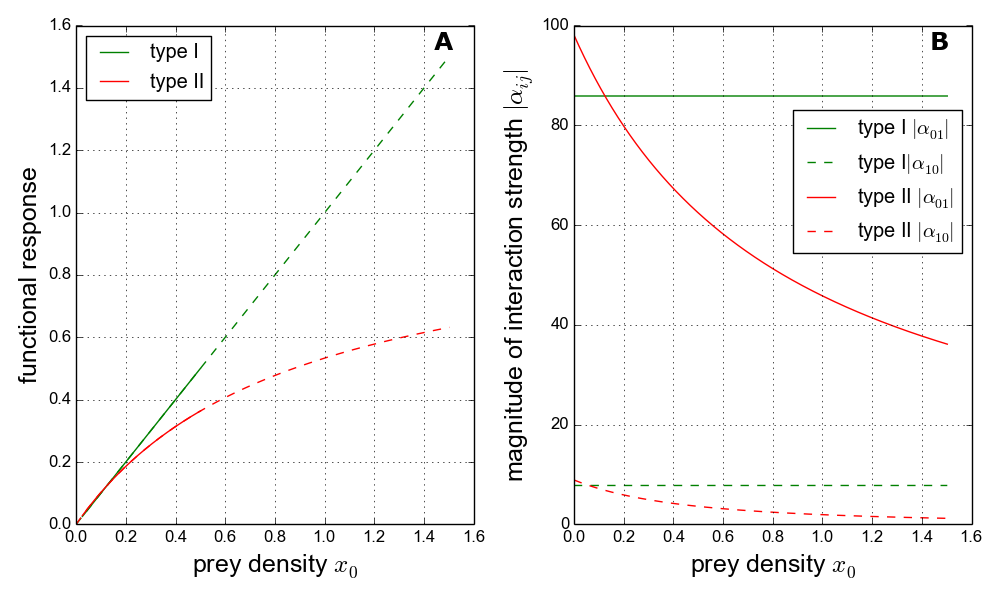
\includegraphics[width=\textwidth]{{{figures/FR_example}}}
\caption{Examples of linear and Holling type II functional responses, and their corresponding interspecific interaction strengths.}
\label{fig:example_FR}
\end{figure}


\newpage
\section{Results}

We run simulations with a range of noise values. 100 parameter sets are chosen such that the deterministic dynamics exhibit two 'large amplitude' oscialltions. We look at how the results of our estimation procedure are affected by noise and by the number of samples taken form the dynamics. 

\begin{figure}[ht!]
\centering 
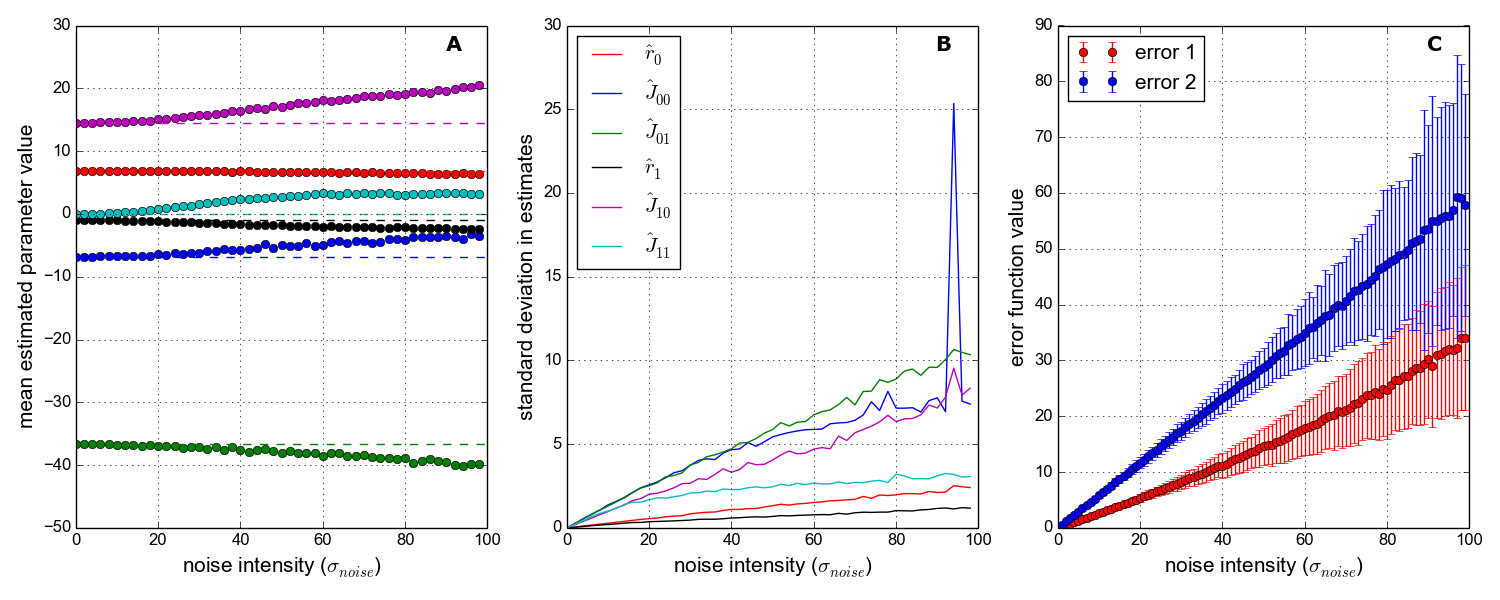
\includegraphics[width=\textwidth]{{{figures/single_params_v_noise_pID_0_nsamples_100}}}
\caption{Results for single parameters set at varying noise levels using 100 samples from simulated dynamics. 1000 repeats at each noise level.}
\label{fig:sp_v_n_100}
\end{figure}

\begin{figure}[hb!]
\centering 
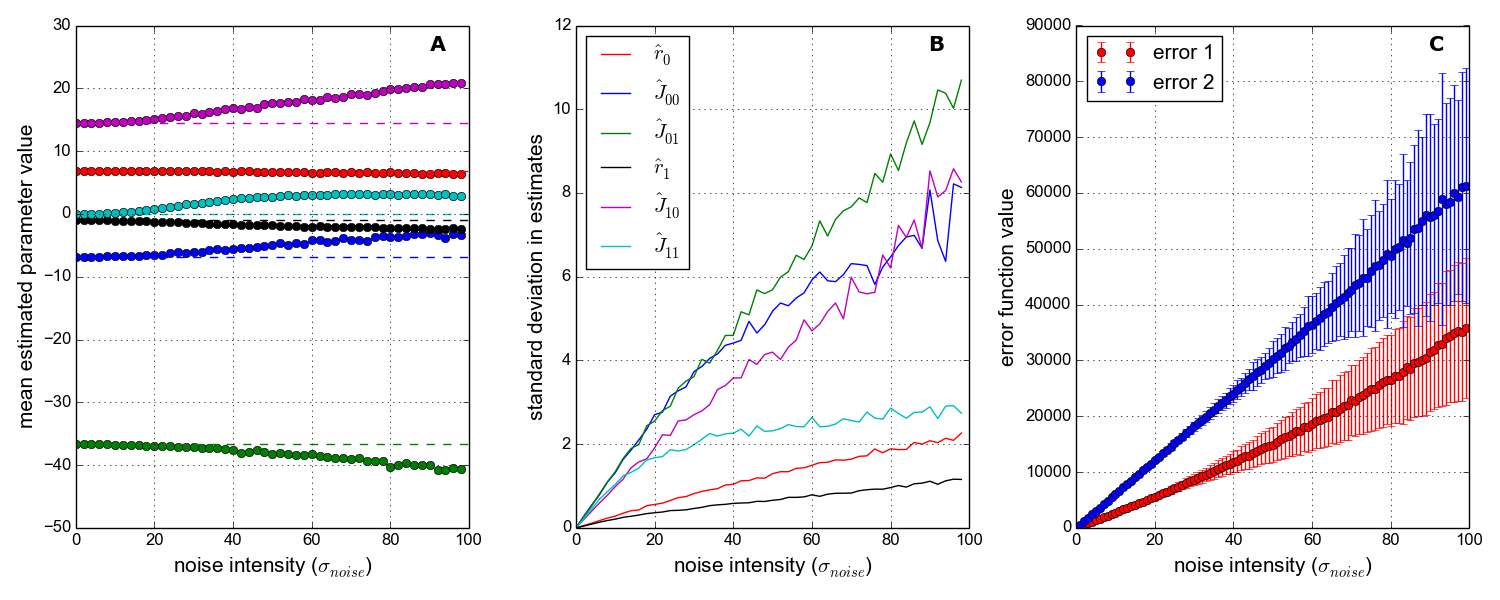
\includegraphics[width=\textwidth]{{{figures/single_params_v_noise_pID_0_nsamples_10000}}}
\caption{As in figure \ref{fig:sp_v_n_100} but using 10,000 samples from the dynamics.} 
\label{fig:sp_v_n_10000}
\end{figure}

\newpage

\begin{figure}[ht!]
\centering 
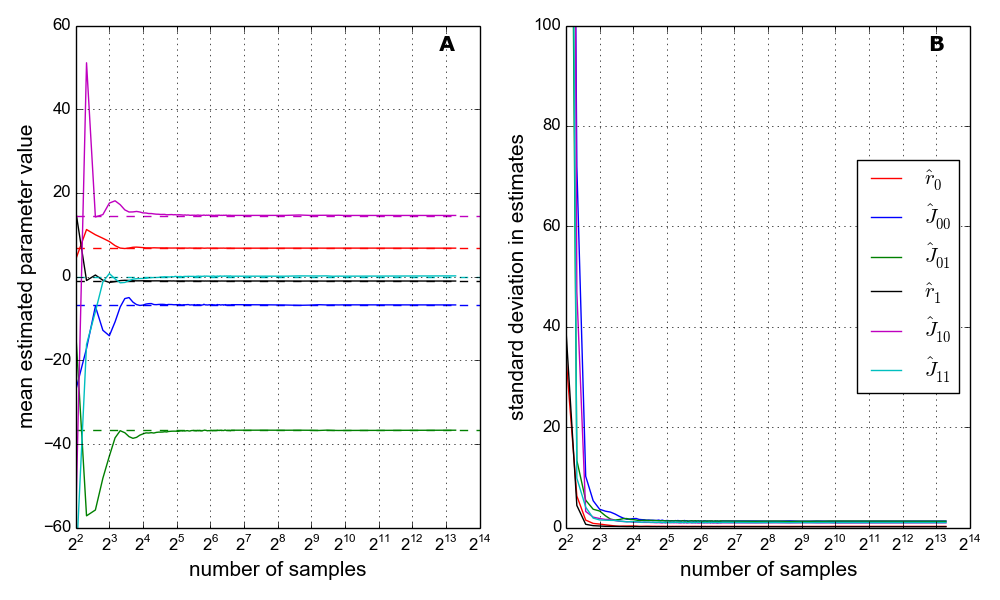
\includegraphics[width=\textwidth]{{{figures/single_params_v_nsamples_pID_0_noise_10.000000}}}
\caption{Results for single parameters set using different numbers of samples from the dynamcis. $\sigma_{noise}=10$. 1000 repeats for each number of samples.}
\label{fig:sp_v_ns_10}
\end{figure}

\begin{figure}[hb!]
\centering 
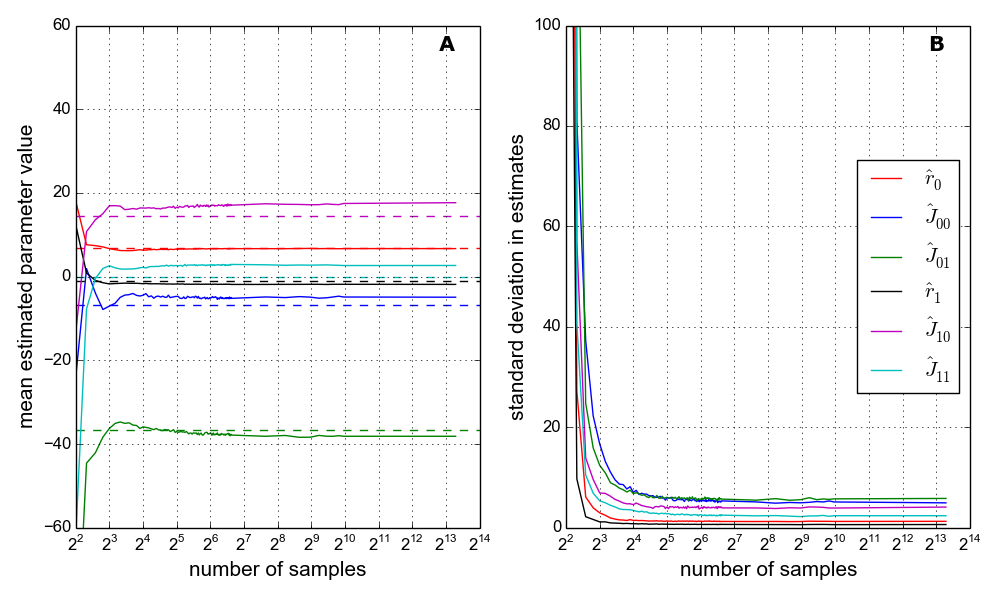
\includegraphics[width=\textwidth]{{{figures/single_params_v_nsamples_pID_0_noise_50.000000}}}
\caption{As in figure \ref{fig:sp_v_ns_10} but with $\sigma_{noise}=50$} 
\label{fig:sp_v_ns_50}
\end{figure}

\newpage

\begin{figure}[ht!]
\centering 
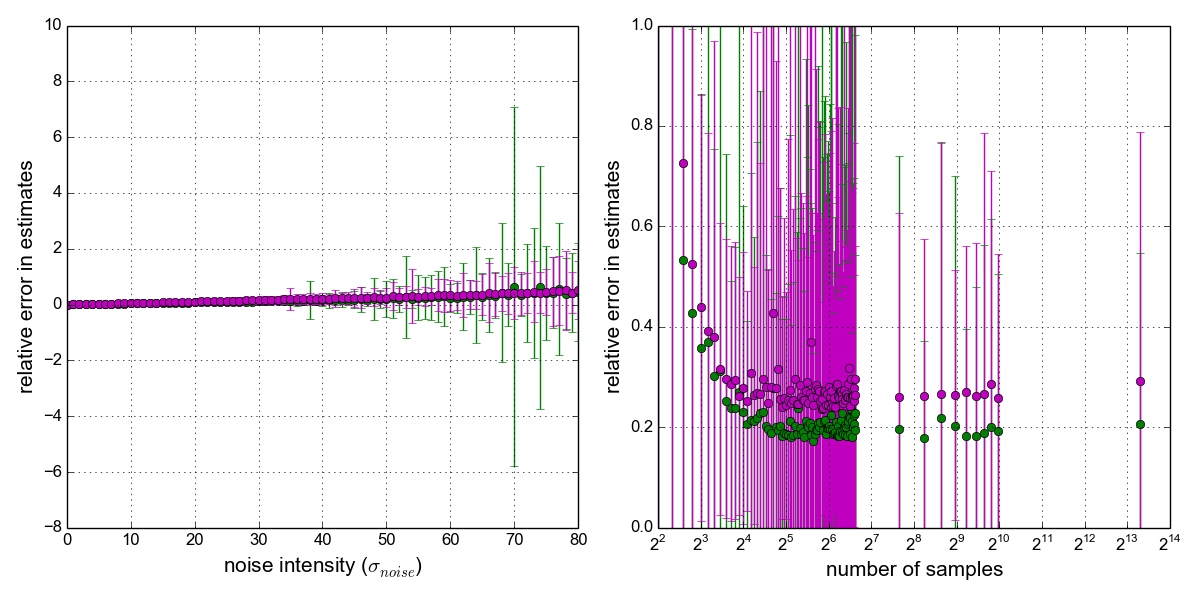
\includegraphics[width=\textwidth]{{{figures/ensemble_results_linear_noise_50.000000_nsamples_1000}}}
\caption{Results for ensemble of parameter sets. Circles showing the expected relative errors in $\hat{J}_{01}$ and $\hat{J}_{10}$. Errorbars showing $\pm$ one standard deviations. 10 repeats for each of 100 parameter sets. For the left plot 1000 samples are used. For the right plot the $\sigma_{noise}=50$.}
\label{fig:en_res_n_50_s_1000}
\end{figure}

\begin{figure}[hb!]
\centering 
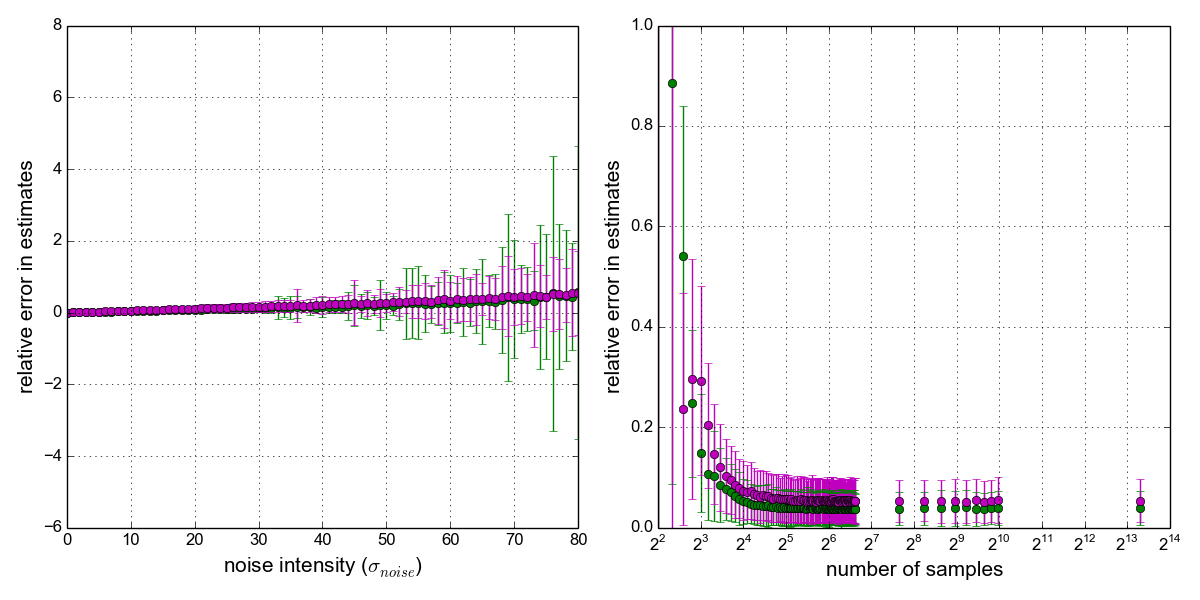
\includegraphics[width=\textwidth]{{{figures/ensemble_results_linear_noise_10.000000_nsamples_10000}}}
\caption{As in figure \ref{fig:en_res_n_50_s_1000} but for the left plot 10000 samples are used, and for the right plot the $\sigma_{noise}=10$.} 
\label{fig:en_res_n_10_s_1000}
\end{figure}

\newpage
\section{Individual based model}

\begin{figure}[ht!]
\centering 
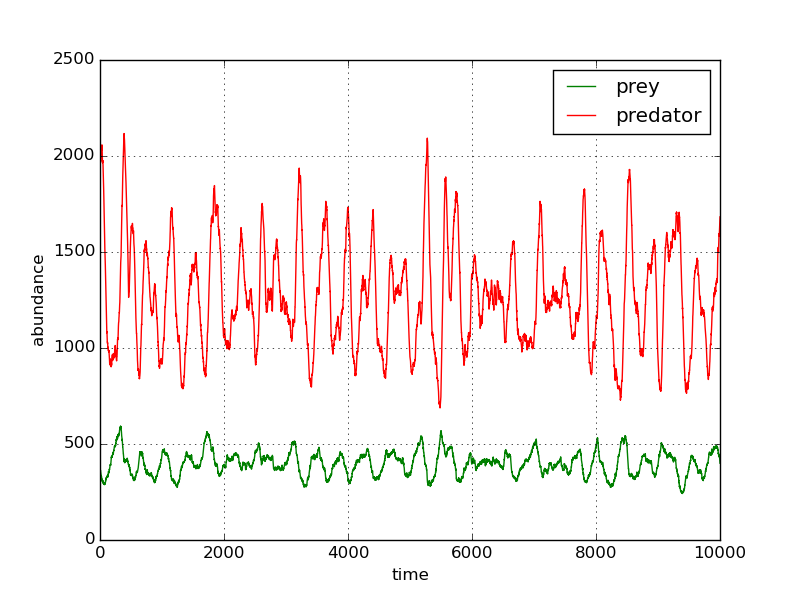
\includegraphics[width=0.6\textwidth]{{{figures/IBM_dynamics}}}
\caption{Examples dynamics of a 2 species predator prey simulation using the IBM model. Run for 10,000 iterations after transience.}
\label{fig:IBM_dynamics}
\end{figure}

\begin{figure}[bt!]
\centering 
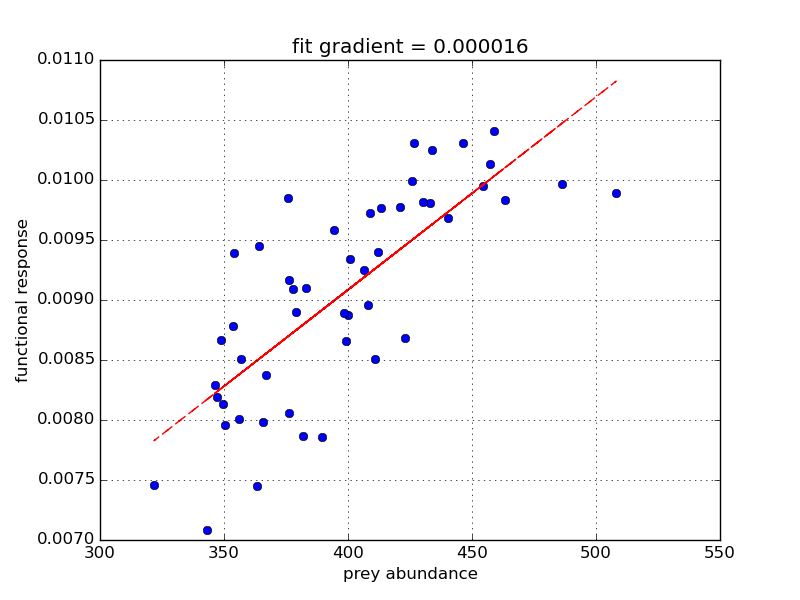
\includegraphics[width=0.6\textwidth]{{{figures/IBM_FR}}}
\caption{The functional response curve, estimated from the dynamics in figure \ref{fig:IBM_dynamics}. Each circle represents the average number of prey consumed per predator per unit time during a window of 200 iterations. A linear fit gives the gradient, which should be equal to the interaction strength.}
\label{fig:IBM_FR}
\end{figure}

\newpage

\begin{figure}[ht!]
\centering 
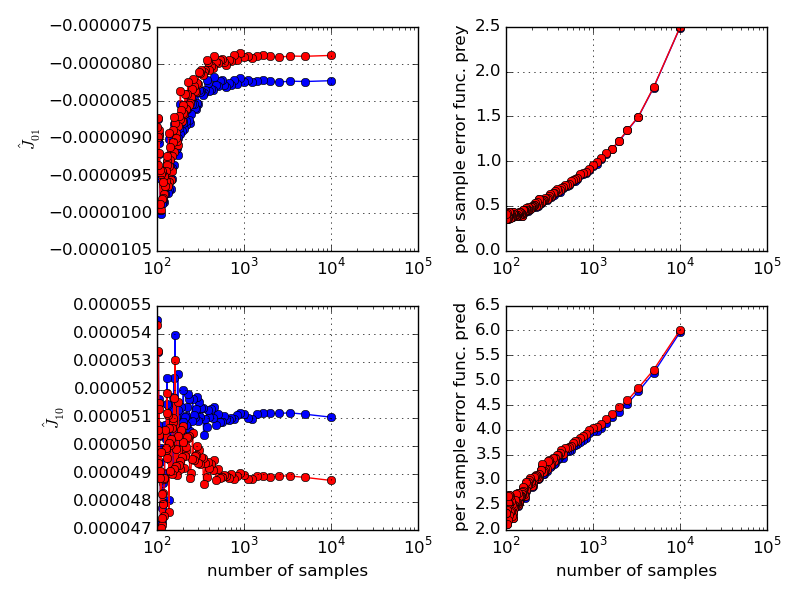
\includegraphics[width=\textwidth]{{{figures/IBM_vs_nsamples}}}
\caption{Results from the simulation run shown in figure \ref{fig:IBM_dynamics}. The left panels show the estimates of the interspecific interaction strengths for increasing sampling frequency. The right hand panels show the value of the error function for each species. The estimates appear to converge, but not to the 'correct' value, as calculated from figure \ref{fig:IBM_FR}.}
\label{fig:IBM_vs_nsamples}
\end{figure}




\end{document}

